\documentclass[boxes]{gsypset}

% Info for header
\mailbox{}
\initials{}
\collaborators{}
\class{Math 65}
\assignment{HW 7}
\duedate{May 25, 2016}

\usepackage{hyperref}
\definecolor{paleviolet}{rgb}{0.8,0.7,0.8}

\begin{document}
	\begin{problem}
		For each system of DEs shown below, explain whether it is
		\begin{itemize}
			\item linear or nonlinear
			\item homogeneous (undriven) or inhomogeneous (driven)
			\item autonomous or nonautonomous.
		\end{itemize}
		Also, for any linear system of DEs, rewrite the system using vector \&
		matrix notation.
		\begin{subproblems}
			\subproblem
				$\begin{cases}
					x'&\hspace{-.1in}=\sin(t)x+e^{ty}y+3t^2 \\
					y'&\hspace{-.1in}=\cos(t)x+e^{-ty}y
				\end{cases}$
				\begin{solution}
					
				\end{solution}
			\subproblem
				$\begin{cases}
					x'&\hspace{-.1in}=3x+4xy \\
					y'&\hspace{-.1in}=2x-3xy
				\end{cases}$
				\begin{solution}
					
				\end{solution}
			\subproblem
				$\begin{cases}
					x'&\hspace{-.1in}=3tx+4ty\\
					y'&\hspace{-.1in}=6t^2x+\sin(t)y
				\end{cases}$
				\begin{solution}
					
				\end{solution}
			\subproblem
				$\begin{cases}
					x'&\hspace{-.1in}=3x+4y+\sqrt{t}\\
					y'&\hspace{-.1in}=\mbox{\hspace{4.5mm}}-3y-\sqrt{t}
				\end{cases}$
				\begin{solution}
					
				\end{solution}
			\subproblem
				$\begin{cases}
					x'&\hspace{-.1in}=3x+2y\\
					y'&\hspace{-.1in}=-x-y
				\end{cases}$
				\begin{solution}
					
				\end{solution}
		\end{subproblems}
	\end{problem}
	
	\begin{problem}
		Here is a general $n$th-order ODE for $y(x)$.
		\[
			a_n(x)\frac{d^ny}{dx^n} +
			a_{n-1}(x)\frac{d^{n-1}y}{dx^{n-1}} +
			\cdots+a_1(x)\frac{dy}{dx} +
			a_0(x)y(x)
			= 0
		\]
		Write it as a system of first-order ODEs, in matrix form.
	\end{problem}
	\begin{solution}
		
	\end{solution}
	
	\begin{problem}
		Consider the second-order ODE $y"(t)+2y'(t)+2y(t)=0$.
		\begin{subproblems}
			\subproblem
				First, solve this ODE using techniques that you learned in Math 45. 
				Express the general solution in two forms: 
					(1) complex exponentials and 
					(2) sines and cosines (with no complex numbers).
				\begin{solution}
					
				\end{solution}
			\subproblem
				Next, convert this second-order ODE to an equivalent first-order DE system. 
				Find the general solution to this system of equations. 
				Use Euler's Identity to rearrange things so that you get a real-valued solution in the end. 
				You should find that your work agrees with your answer from part (a).
				\begin{solution}
					
				\end{solution}
		\end{subproblems}
	\end{problem}
	
	\begin{problem}
		Solve the initial-value problem $\mathbf{x}'(t)=A\mathbf{x}(t)$
	  with $A = \bm{5 & 5 & 2 \\ -6 & -6 & -5 \\ 6 & 6 & 5}$ and
		$\mathbf{x}(0) = \bm{1 \\ -1 \\ 1}$.\\
		Express your answer as a real-valued function.
	\end{problem}
	\begin{solution}
		
	\end{solution}
	
	\begin{problem}
		At $t=0$ (i.~e.~noon) a student takes a fast-dissolving antihistamine capsule. 
		The antihistamine is absorbed from the GI tract (stomach and intestines) 
		into the blood system and then excreted. 
		Let $x_1$ be the amount of antihistamine in the GI tract and 
		$x_2$ be the amount in the blood system. 
		Assume that the rate of absorption from the GI tract into the blood system is $k_1x_1$ 
		and the rate of excretion from the bloodstream (via the kidneys) is $k_2x_2$, 
		corresponding to the following compartment diagram. 
		Also, assume that $k_2<k_1$ (the rate of excretion is faster than the rate of absorbtion).
		\begin{center}
			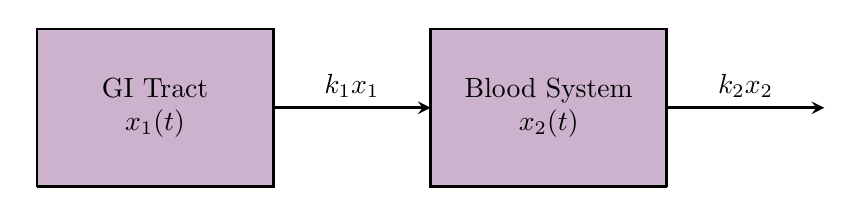
\begin{tikzpicture}[scale=2]
				\draw [fill=paleviolet,line width=1]
					(-1.5,-0.5) -- (0,-0.5) -- (0,0.5) -- (-1.5,0.5) -- (-1.5,-0.5);
				\draw (-0.75,0) node[text width=3cm,align=center] {GI Tract\\$x_1(t)$};
				\draw[line width=1,>=stealth,->] (0,0) -- (1,0) node[above,midway] {$k_1x_1$};
				\draw [fill=paleviolet,line width=1]
					(2.5,-0.5) -- (1,-0.5) -- (1,0.5) -- (2.5,0.5) -- (2.5,-0.5);
				\draw (1.75,0) node[text width=3cm,align=center] {Blood System\\$x_2(t)$};
				\draw[line width=1,>=stealth,->] (2.5,0) -- (3.5,0) node[above,midway] {$k_2x_2$};
			\end{tikzpicture}
		\end{center}
		\begin{subproblems}
			\subproblem
				Explain why the amount of antihistamine in the body satisfies the system
				\begin{align*}
					\frac{dx_1}{dt} &=  -k_1 x_1 \\
					\frac{dx_2}{dt} &= k_1 x_1 -k_2 x_2
				\end{align*}
				together with the initial conditions $x_1(0)=\alpha$ and $x_2(0)=0$
				where $\alpha$ is the initial amount of antihistamine in the GI tract 
				just after the capsule has dissolved.
				\begin{solution}
					
				\end{solution}
			
			\subproblem
				This system of equations is a \textit{cascading} system of equations 
				in that the first equation only involves $x_1$ and 
				the second equation involves both $x_1$ and $x_2$. 
				Therefore, you can solve the first equation by itself, 
				then plug in the solution for $x_1$ into the second equation and solve for $x_2$. 
				Solve the system in this fashion.
				\begin{solution}
					
				\end{solution}
			
			\subproblem
				Next solve the system of equations again using linear algebra 
				(eigenvalues and eigenvectors of the system matrix).
				\begin{solution}
					
				\end{solution}
			
			\subproblem 
				When does the amount of antihistamine in the blood system reach a maximum? 
				What is the maximum amount? 
				Your answers will be in terms of $\alpha$, $k_1$, and $k_2$ 
				(\textbf{Hint:} Your final answer for the maximum amount can be written quite simply.)
				\begin{solution}
					
				\end{solution}
		\end{subproblems}
	\end{problem}
	
	\begin{problem}
		Make up an initial-value problem involving a system of 
		linear, first-order differential equations that has the property that 
		its solution exists only for $a<t<b$, where $a$ and $b$ are numbers of your choosing. 
		Use ODEToolkit (\url{http://odetoolkit.hmc.edu}) to draw the solution trajectories. 
		Make sure you label your axes and show that the solution only exists for $a<b<t$.
	\end{problem}
	\begin{solution}
		
	\end{solution}
\end{document}

